\documentclass{standalone}
\usepackage{tikz}
\usepackage{ctex,siunitx}
\setCJKmainfont{Noto Serif CJK SC}
\usepackage{tkz-euclide}
\usepackage{amsmath}
\usetikzlibrary{patterns, calc,3d}
\usetikzlibrary {decorations.pathmorphing,decorations.pathreplacing,decorations.shapes}
\begin{document}
\small
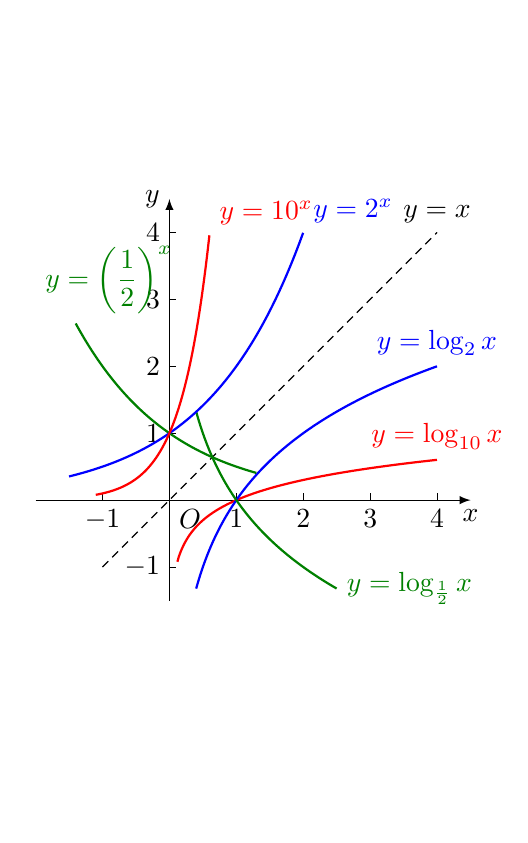
\begin{tikzpicture}[>=latex,scale=1.0]
  \useasboundingbox(-1.8,-4)rectangle(4.2,6);
  \begin{scope}[scale=0.85]
  \draw[->](-2,0)--(4.5,0)node[below]{$x$};
  \draw[->](0,-1.5)--(0,4.5)node[left]{$y$};
  \node at (0,0)[below right]{$O$};
  \draw[densely dashed](-1,-1)--(4,4)node[above]{$y=x$};
  \foreach \x in {1,2,3,4,-1} 
    {
      \draw[very thin](\x,0)node[below]{$\x$}--++(0,0.1);
      \draw[very thin](0,\x,0)node[left]{$\x$}--++(0.1,0);
    }
  \draw[thick,red,samples=200,domain=0.12:4]plot(\x,{log10(\x)})node[above]{$y=\log_{10} x$};
  \draw[thick,blue,samples=200,domain=0.4:4]plot(\x,{log2(\x)})node[above]{$y=\log_2 x$};
  \draw[thick,green!50!black,samples=200,domain=0.4:2.5]plot(\x,{-log2(\x)})node[right]{$y=\log_{\frac12} x$};
  \draw[thick,green!50!black,samples=200,domain=-1.4:1.3]plot(\x,{pow(0.5,\x)});
  \node at (-2.0,{pow(0.5,-1.4)}) [above right,green!50!black]{$y=\left(\dfrac12\right)^x$};
  \draw[thick,blue,samples=200,domain=-1.5:2]plot(\x,{pow(2,\x)})node[above right]{$y=2^x$};
  \draw[thick,red,samples=200,domain=-1.1:0.6]plot(\x,{pow(10,\x)})node[above right]{$y=10^x$};
  \end{scope}
\end{tikzpicture}
\end{document}